%% LyX 2.1.4 created this file.  For more info, see http://www.lyx.org/.
%% Do not edit unless you really know what you are doing.
\documentclass[12pt,english]{article}
\usepackage[T1]{fontenc}
\usepackage[latin9]{inputenc}
\usepackage{wrapfig}
\usepackage{amsmath}
\usepackage{graphicx}
\usepackage[numbers]{natbib}

\makeatletter
%%%%%%%%%%%%%%%%%%%%%%%%%%%%%% Textclass specific LaTeX commands.
\numberwithin{equation}{section}
\numberwithin{figure}{section}

%%%%%%%%%%%%%%%%%%%%%%%%%%%%%% User specified LaTeX commands.
\usepackage{pgfgantt}
\usepackage{adjustbox}
\usepackage{listings}
\usepackage{hyperref}
\hypersetup{pdftex,colorlinks=true,allcolors=blue}
\usepackage{hypcap}
\usepackage{a4wide}
\usepackage[hide]{ed}
\usepackage{graphicx}
\usepackage{onecolpceurws}
\usepackage{paralist}

\title{Notation-based Semantification}
\author{ Toloaca Ion \and Kohlhase Michael}
\institution{Jacobs University Bremen}

\makeatother

\usepackage{babel}
\begin{document}
\maketitle


\section{Introduction}

The scientific community produces a large number of mathematical papers
(approximately $108.000$ new papers per year \citep{arxivSubmission}),
which raises the importance of machine based processing of such documents.
Unfortunately, the most popular formats in which these papers are
found (for instance, \LaTeX{}) do not contain much information that
would allow the computers to infer the human-understandable knowledge
contained within a paper. Since, at this point, changing these formats
is not practically possible, the other solution is to add a semantic
flavor to the existing documents by translating them into a more suitable
format, for instance, Content MathML.

As a system as complex as the current scientific community was created,
it went through a series of evolutions in the attempt to introduce
the best method of writing scientific documents. This process was
highly influenced by the invention and spreading of the internet.
Scientists understood the necessity of a standard that could help
them write and exchange their findings in an efficient way. A lot
of effort has gone into translating books into digital documents. 

The next step in this evolution is translating digital documents into
knowledge-rich digital documents. This next step can only happen if
a new feasible way of transition appears, which \textbf{MathSemantifier
}attempts to become.

An important concept necessary in order to understand why semantification
is a complex process is ambiguity. Mathematical documents are not
a simple collection of symbols. The main use of these documents emerges
only when the intended semantics of a document is accessible. However,
humans tend to be lazy in writing down the whole graph, but instead
rely on implicit human knowledge to decipher these documents. This
is where ambiguity comes into play, when the author relies on the
ability of the human to use the context of document in order to pinpoint
the actual meaning an expression. Ambiguities can be largely divided
into two: structural and idiomatic ambiguities.

A simple example that demonstrates the concept of structural ambiguities
can be $\sin\ x\ /\ 2$. It can mean one of the following:
\begin{enumerate}
\item $\sin$ applied to $\frac{x}{2}$ 
\item $\frac{1}{2}$ times $\sin$ applied to $x$
\end{enumerate}
Contrary to structural ambiguities, idiomatic ambiguities are not
due to different parse trees. Given one single parse tree, some formulae
allow for multiple readings. A standard example would be $B_{n}$.
This could be:
\begin{enumerate}
\item The sequence of Bernoulli numbers
\item A user defined sequence
\item The vertex of one of a series of geometric objects
\end{enumerate}
In this paragraph we propose a solution to the ambiguity problem described
above. Consider $c(a(b))$. The most natural interpretation is $c$
of $a$ of $b$. However, there arise multiple meanings if we consider
that the application could be interpreted as multiplication. The human
reader discards such meanings by convention and experience of handling
mathematical documents, however, teaching this to a computer is a
complex task. The approach that \textbf{MathSemantifier }takes is
simply extracting all the possible meanings, while trying to apply
heuristics to weed out impossible meanings.


\subsection{An Introduction to MathSemantifier}

In order to understand what \textbf{MathSemantifier }does, the Presentation
Algorithm needs to be explained first. The reason for that is that
\textbf{MathSemantifier }is the exact opposite of the Presentation
Algorithm, trying to convert PMML to CMML, as opposed to CMML to PMML.

The presentation algorithm has its main goal to covert Content MathML
to Presentation MathML, using a database of notation renderings. In
\autoref{fig:presentation_output} a typical example of what the presentation
algorithm produces is displayed. The\textbf{ }first child of the \textbf{semantics
}node contains the PMML that corresponds to the CMML contained in
the \textbf{annotation-xml }node. In order to produce this output,
the algorithm used the notation \textbf{natarith addition (}shown
in \autoref{fig:presentation_output} as well). OMDoc Notations like
\textbf{natarith addition }are initially written in s\TeX{}, and then
converted to OMDoc using \LaTeX{}ML.

\begin{figure}
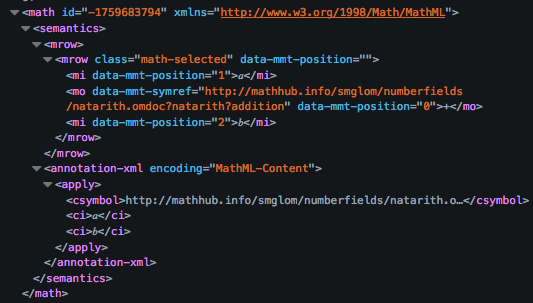
\includegraphics[bb=0bp 0bp 533bp 300bp,clip,width=8cm,height=5cm]{present_math}\hspace{0.3cm}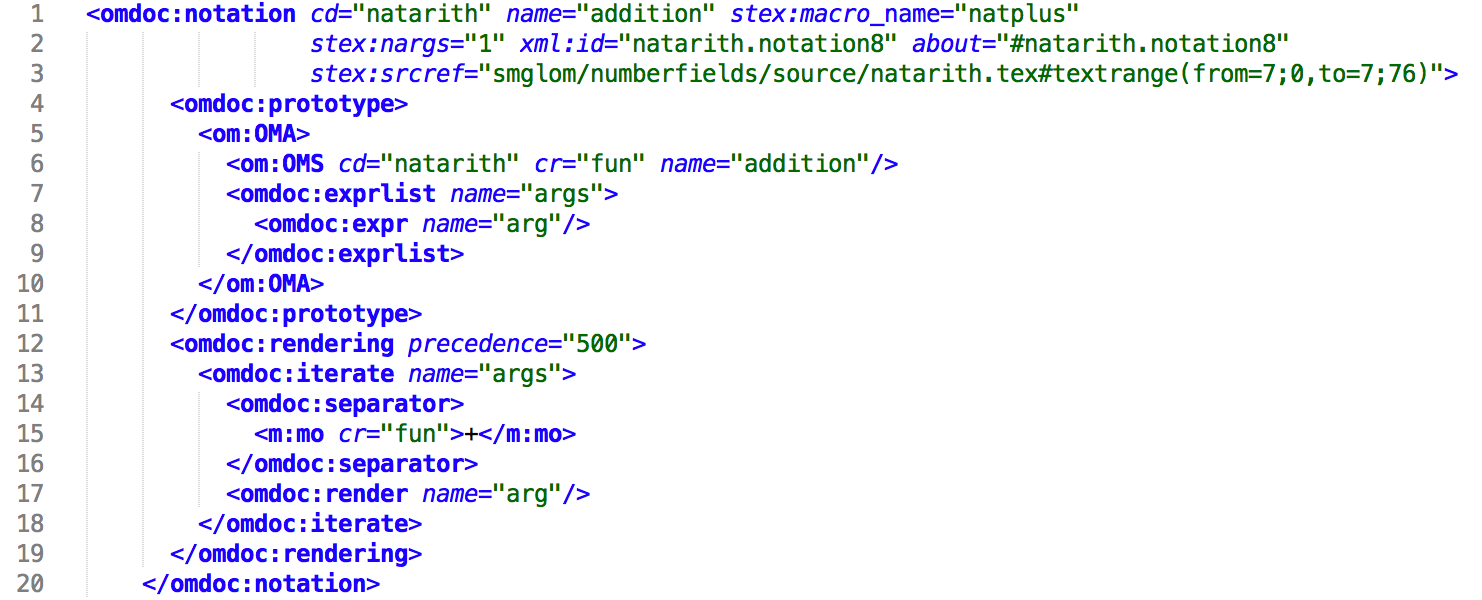
\includegraphics[width=9cm,height=5cm]{presen_not}\caption{Presentation Algorithm Output and the corresponding Notation Definition\label{fig:presentation_output}}
\end{figure}


\textbf{MathSemantifier }converts PMML into valid CMML as described
above. In order to perform this task, it needs to match PMML against
a list of notations. This is achieved by compiling the notations into
a Context Free Grammar, and using a CFG Parsing Engine to parse the
PMML. A parse returns a list of possible parse trees, out of which
\textbf{MathSemantifier }extracts information regarding what notations
matched at top level. This is then done recursively for the arguments
of the found notation. Parsing using CFGs is a known problem, so,
instead of writing a Parsing Engine, a more reasonable approach is
using an existing one. For that purpose, the \textbf{Marpa Grammar
Engine }is used.

Possible Applications of Semantification include:
\begin{itemize}
\item \textbf{MathWebSearch \citep{MWS12}} is a search engine for mathematical
formulas. Such search engines could greatly benefit from semantification.
The idea is that a search engine is only as good as the database of
information is. By improving the information it can search through
by adding a semantic flavor to it, a new kind of queries could be
possible - semantic queries. Rather than searching for strings, or
formulas with free form subterms, the user could specify the meaning
of the sought expression. This would improve a lot the relevance of
the results, since there will be no result that matched just because
it was presented in a similar manner. 
\item Another possibility for using semantification is theorem proving and
correctness checking. One possible application would be realtime feedback
to the user writing a paper about the correctness of the expressions
used.
\item The possibilities extend even beyond this. Using semantified content,
rather than having a database of CMML expressions, it is possible
to create a smart knowledge management system that could be used to
create expert systems. The user could then ask questions, or create
complex queries, to exploit the full power of semantic content.
\end{itemize}
Semantification will not make all of the above directly possible,
however it is a necessary step towards achieving goals similar to
the ones described above, that require more knowledge about the used
content than just how it is rendered.

MathSemantifier uses a Notation Database to create the grammar it
uses. Therefore, it needs to be explained where those notations come
from. MMT \citep{MMT} is a language developed as a scalable representation
and interchange language for mathematical knowledge. The decisive
factor about MMT is that there is already a large database of notations
written in s\TeX{}, which is transformed and stored in MMT in an original
format that MathSemantifier is processing in order to generate a Context
Free Grammar.

SMGloM \citep{SMGLOM} is a part of the notation database of MMT that
contains the notations used by \textbf{MathSemantifier}. SMGloM is
also available online \citep{smglomweb}.

Since s\TeX{}, as an extension of \LaTeX, is just as complex to parse,
MMT uses \LaTeX{}ML in order to convert s\TeX{} to OMDoc \citep{OMDOC}.
OMDoc is then processed and stored in MMT. 

\textbf{MathSemantifier} takes the auto-generated CFG and input from
the \textbf{Web UI} in order to produce possible parse trees of the
input. Marpa Grammar Engine is the proposed. The main advantages are
that Marpa handles ambiguous grammars and provides control over the
parsing process. The author of Marpa provides a more detailed analysis
of the advantages of Marpa (see \citep{marpaParser}).


\section{The MathSemantifier System}

The major idea of \textbf{MathSemantifier }is, as already described
in the introduction, finding possible Content MathML readings for
Presentation MathML input expressions. 

The general flow of a single semantification can be described as follows:
\begin{enumerate}
\item Context Free Grammar generation from the MMT Notations 
\item Parsing using the Marpa Grammar Engine and the generated CFG to detect
the top level notation
\item Parsing the arguments of the top level notation recursively
\item Using the parse trees from step 2 and 3 to generate an internal representation
of the meaning trees
\item Converting the meaning trees to Content MathML
\item Displaying the Content MathML trees in the frontend
\end{enumerate}
The reason it was decided to use a CFG based solution is that there
exist already parsing frameworks like the Marpa Grammar Engine. It
solves all the parsing related technical problems, like parsing ambiguous
expressions, different kinds of recursion, while also providing a
high degree of freedom. 

This sections goes into the details of how exactly semantification
is accomplished. First, a general overview of the goals of the project
and its high level architecture is given. Then, each component is
described in further detail.

The main goals of the project can be expressed in a concise manner
as follows:
\begin{enumerate}
\item Generating the correct set of parses efficiently and effectively
\item Providing opportunities for improvement for further research in the
area
\end{enumerate}
The architecture can be roughly divided into four parts as shown in
\autoref{fig:7}. 

\begin{figure}
\hspace{2cm}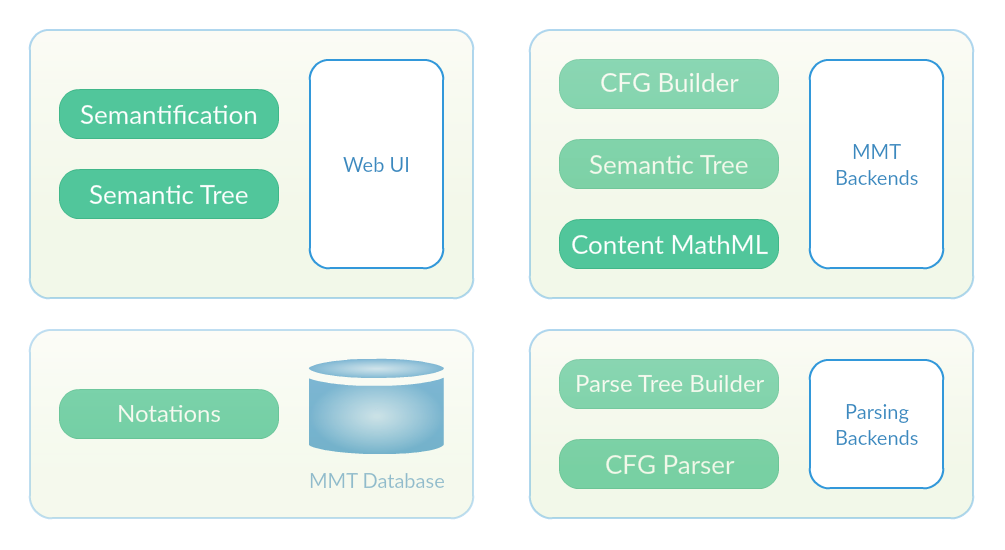
\includegraphics[width=12cm]{myThesisComponents_diagram}\caption{\textbf{MathSemantifier} Architecture \label{fig:7}}
\end{figure}


The \textbf{Web UI }is a core component of \textbf{MathSemantifier.}
It is intended to be a lightweight solution that queries a server
for the results of more computationally intensive tasks.

The interface consists of an input area, where \textbf{MathML }needs
to be inputted, and three options:
\begin{enumerate}
\item Semantify (The user can guide the semantification of the top symbol
directly, by choosing the correct matching range, notation and argument
positions)
\item Show Semantic Tree (The other option is to ask for all the possibilities
and get all the semantic trees)
\item Evaluation (In this case, by repeatedly pressing this, the user is
walked through a series of examples to demo the functionality)
\end{enumerate}
The repository containing the \textbf{Web UI }can be found on GitHub
\citep{codeWebUI}.

User Guided Semantification is performed as follows: The user provides
Presentation MathML as input to the system, then uses the \textbf{Semantify
}button to reveal a list of top level notation names. The names of
the notations are derived from the notation paths as follows: \textbf{archive
name} + \textbf{symbol name}, for example, \textbf{natarith addition
}refers to the addition of natural numbers. After determining which
notation is the correct one, the user needs to make sure that the
arguments were detected properly and, finally, the resulting Content
MathML tree is displayed (see \autoref{fig:6} for a similar representation
of the result).

The easier but computationally more expensive alternative is to simply
generate all the possible parse trees at once and display them. The
user simply needs to click the \textbf{Show Semantic Tree} option.

\begin{wrapfigure}{o}{0.5\columnwidth}%


\vspace{-1.5cm}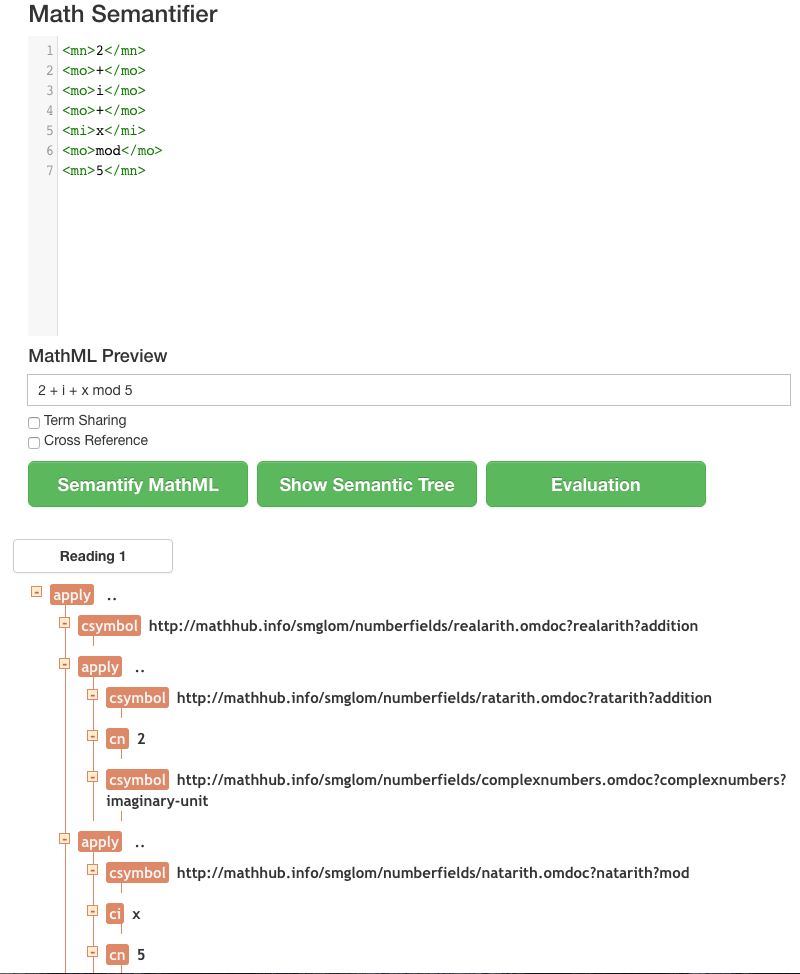
\includegraphics[bb=0bp 5bp 800bp 972bp,clip,width=10cm]{auto1}\caption{\label{fig:6}}


\end{wrapfigure}%


For the example shown in \autoref{fig:6}, there is a total of 342
different readings. This can be easily explained, since \textbf{Invisible
Times}, \textbf{Arithmetic Plus} and \textbf{Mod }have each multiple
notations definitions (that originate from different MMT archives,
for instance), and there are no limitations on what kind of notation
definitions can go together in the same CMML tree.

In order to minimize the Content MathML, the standard allows subtree
sharing. To enable this option, the \textbf{Use term sharing }checkbox
should be checked. In that case, the terms is shared along different
readings.



The MMT Backend is a \textbf{Server Extension }that is part of MMT.
As shown in \autoref{fig:7}, it is linked via \textbf{REST} with
the \textbf{Web UI }and the \textbf{Parsing Backends.} 

Its role can be summarized to the following core functions:
\begin{enumerate}
\item Compile the \textbf{MMT Notations} into a CFG Grammar
\item Receive the input from the \textbf{Web UI} and build its Semantic
Tree
\item Delegate the parsing to the \textbf{Parsing Backends}
\end{enumerate}
I decided to put the core logic of the application in MMT in order
to make it easier to interoperate with the MMT Notation Database,
as well as with any other MMT components that may want to need \textbf{MathSemantifier.}
By the current design, using \textbf{MathSemantifier }within MMT is
as simple as a function call that takes the input as a string.

The code can be found as part of the MMT codebase \citep{codeMMT}.

Let us look at the components of the MMT Backends in more detail below.

\vspace{0.1cm}

The Grammar Generator aggregates all the knowledge contained in the
MMT Notations into one Context Free Grammar. The grammar is shaped
into the normal form accepted by the Marpa Grammar Engine. To achieve
this, the format used to store the notations in MMT is decomposed
into CFG rules. Otherwise said, the tree-like structure of each formula,
that is stored as nested applications of \textbf{MMT Markers} needs
to be serialized into CFG rules.

\begin{wrapfigure}{o}{0.5\columnwidth}%
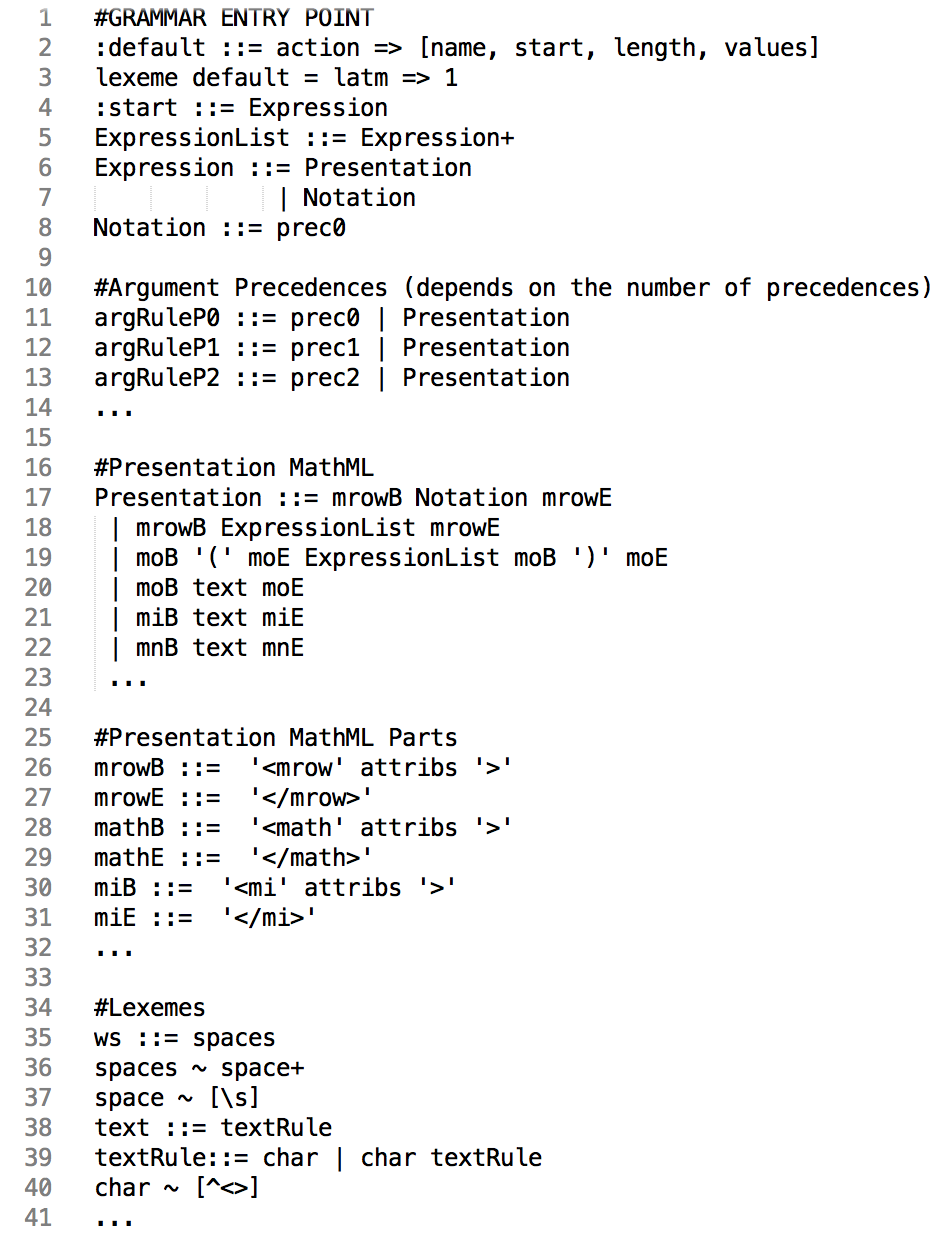
\includegraphics[width=8cm]{cfg_preamble}

\caption{CFG Preamble\label{fig:cfg_preamble}}
\end{wrapfigure}%


This is done in several steps:
\begin{enumerate}
\item Break apart the \textbf{MMT Marker }trees into level by level representations
\item Transform the intermediate representation into valid CFG rules
\end{enumerate}
The fundamental structure of the CFG is established using a preamble
as shown in \autoref{fig:cfg_preamble}. Note the default action is
the \textbf{Grammar Entry Point.} It is precisely what tells the Grammar
Engine to build parse trees, and also determines their structure.

The entry point into the grammar is the \textbf{Expression }rule.
It can be an MMT Notation, or Presentation MathML. The \textbf{prec0}
rule should be read as precedence zero, that is - the lowest precedence
there is.

\begin{wrapfigure}{o}{0.5\columnwidth}%
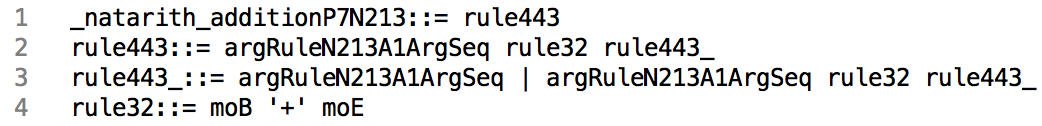
\includegraphics[width=10cm]{cfg_ex}\caption{MMT Notation in CFG\label{fig:cfg_ex}}
\end{wrapfigure}%


Precedence handling is done using a commonly used method for including
it in CFGs. The \textbf{Notation Precedences }section in \autoref{fig:cfg_preamble}
gives a quick glance at how exactly it is done. The number of precedences
needs to be known in advance, then, for each precedence value a corresponding
\textbf{precN} rule is created.

The rule contains all the notations with that precedence, and, one
of the alternatives is going to a higher precedence value. In the
example below there are 15 used precedence values (\textbf{prec0 }corresponds
to precedence $-\infty$). However, the \textbf{Notation Precedences
}section shows only half of the concept.

To make this approach work, what is also needed is that the arguments
in a rule of a certain precedence N can only contain notations with
precedence $K$ if $K>N$. This is done by the \textbf{Argument Precedences
}part in the preamble (as shown in \autoref{fig:cfg_preamble}).

Finally, \autoref{fig:cfg_ex} presents an example of what the \textbf{natharith
addition }MMT notation from the \textbf{smglom/numberfields }archive
translated to CFG rules looks like.

The \textbf{Semantic Tree Generator }works by recursively querying
the \textbf{Parsing Backend }and using the result to construct the
tree of possible meanings.

The parse trees stored in MMT have the following structure:
\begin{itemize}
\item \textbf{Variants - }represents a list of possible readings. It is
always the top node in any parse tree.
\item \textbf{Notation - }a notation detected in the input. It contains
its name and arguments.
\item \textbf{Argument - }an argument of a notation. The plugin is recursively
called on it to construct its meaning subtree as well.
\item \textbf{RawString - }the ground term representation
\end{itemize}
The final part of the semantification processes is converting the
internal representation to a standard one, which is CMML in this case.
MMT provides a simple API which requires:
\begin{enumerate}
\item The MMT notation path
\item The argument maps (maps from the argument number to the corresponding
substring)
\end{enumerate}
Both of which are available in my representation structure. The argument
path is obtained by extracting the argument number from the argument
name, and looking up in a map of paths created at the time of grammar
creation. This implies the grammar rule names are overloaded with
meaning, however, the possibilities are very limited in this aspect
since the parsing framework used does not give complete control over
the parsing process.

The Parsing Backend \autoref{fig:7} receives requests from the \textbf{Web
UI }directly for Guided Semantification and from the \textbf{MMT Backend
}for Semantic Tree Generation. All the parsing related work is delegated
to this backend.

The code of the Parsing Backend can be found on GitHub \citep{codeParsingBackend}.

The parsing backend consists of two parts. 

First of all, the CFG needs to be queried and parsed. This is implemented
using lazy evaluation, which means that it is only done when a request
actually comes.

The serialized CFG is unpacked and feed to the Marpa Parser Generator.

The more complex of the two parts is actually going through the parse
trees and extracting useful information. Note that going through all
the parse trees is not practical, so only the first $N$ (currently
$1000$) parse trees are processed. This still gives the correct results
in most cases since the grammar rules are optimized for giving preference
to parse trees that are more likely to be correct.


\section{\label{8}Evaluation }

This section presents an evaluation of \textbf{MathSemantifier }from
the point of view of efficiency and effectiveness of semantic tree
generation. Next, the interoperability of the system with other possible
applications is examined, which mostly depends on the backend APIs.

Testing \textbf{MathSemantifier} through normal operation is not a
trivial task, because the results need a human expert to check whether
the results are indeed correct. Fortunately, the \textbf{MathHub Glossary
\citep{glossary}} contains a sufficient number (about 3000) of examples
of Presentation MathML with Content MathML annotations that result
from applying the \textbf{Presentation Algorithm} discussed in the
introduction. Since \textbf{MathSemantifier }is the partial inverse
of the \textbf{Presentation Algorithm, }checking whether the results
are indeed correct boils down to comparing two Content MathML trees.

For the purpose of testing \textbf{MathSemantifier} on the \textbf{MathHub
Glossary, }the \textbf{Evaluation }option mentioned in the \textbf{Web
UI} section is used. It processes examples from the \textbf{MathHub
Glossary. }

A visual control of approximately 500 examples from the \textbf{MathHub
Glossary} revealed the following results\textbf{. }About 40\% of the
examples are semantified correctly. However, this is largely because
of reasons that do not depend on \textbf{MathSemantifier} itself.

Contrary to what the numerical result suggests, for expressions with
less than 1000 parse trees that are correctly rendered, \textbf{MathSemantifier
}produces correct results with a very high probability.

Let us look into the reasons that make \textbf{MathSemantifier }fail.
First of all, the reasons that do not depend on the system itself.
\begin{enumerate}
\item The Presentation Algorithm fails to render CMML into PMML properly
in about 30-40\% of the cases.
\item About 10\% of the examples include symbols from archives that were
not included in the CFG
\end{enumerate}
Up to this point, if we exclude the above mentioned examples, the
effective success rate of \textbf{MathSemantifier} is about 80-90\%.
\begin{enumerate}
\item Some notations are omitted because they create cycles in the CFG
\item Input data that is too long or complex having more than 1000 parse
trees
\item Assuming the input is more knowledge-rich than it actually is
\end{enumerate}
While the effective success rate of 80-90\% is inspiring for a proof
of concept system, the main issue of \textbf{MathSemantifier }is simply
poor performance on long or complex input. Therefore, \textbf{MathSemantifier}
is a successful proof of concept, but not yet a practical tool.


\section{Conclusions }

The conclusion of this study is the proof of concept architecture
and implementation of a system capable of converting \textbf{Presentation
MathML} to all the possible meanings, which is a list of \textbf{Content
MathML}. The testing revealed that the system is able to recognize
correctly single top level symbols, as well as the whole set of readings
of expressions with less than 1000 parse trees (this is not the limit,
but no testing is done beyond that). Naturally, \textbf{MathSemantifier
}can only recognize the symbols that were used when building the Context
Free Grammar it uses. This shows that it is certainly possible to
aggregate the knowledge from the MMT Notations and to use it for parsing
purposes. However, both the Notations and the Parsing Framework need
significant improvements in order for the system to be scalable beyond
what is presented in the previous section. The most important part
of this study is, therefore, the optimizations and heuristics used,
and other techniques presented below that further research could benefit
from.

\bibliographystyle{alpha-fr}
\addcontentsline{toc}{section}{\refname}\bibliography{bibtexDatabase}

\end{document}
